\chapter{Introducción}\label{cap:introduccion}

El mundo de la robótica está en pleno auge, y cada vez es más común encontrar robots en nuestro entorno cotidiano. Ya sea porque conocemos a alguien que tiene un robot aspirador, hemos visto noticias sobre avances tecnológicos, o incluso hemos interactuado directamente con alguno, su presencia resulta cada vez más habitual.

\section{Robótica de Servicio}

Entre los más comunes se encuentran los robots de servicio, aquellos diseñados para asistir a los humanos en tareas específicas. En este grupo se incluyen dispositivos como aspiradoras autónomas (\autoref{fig:roomba}), robots logísticos como los AGV (vehículos de guiado automático, \autoref{fig:agv}) y los AMR (robots móviles autónomos, \autoref{fig:amr}), drones de rescate (\autoref{fig:dron}), el robot \textit{Da Vinci}\footnote{\url{http://www.icirugiarobotica.com/cirugia-robotica-da-vinci/}} que ayuda a los cirujanos (\autoref{fig:davinci}), etc.

\begin{figure}[H]
    \centering
    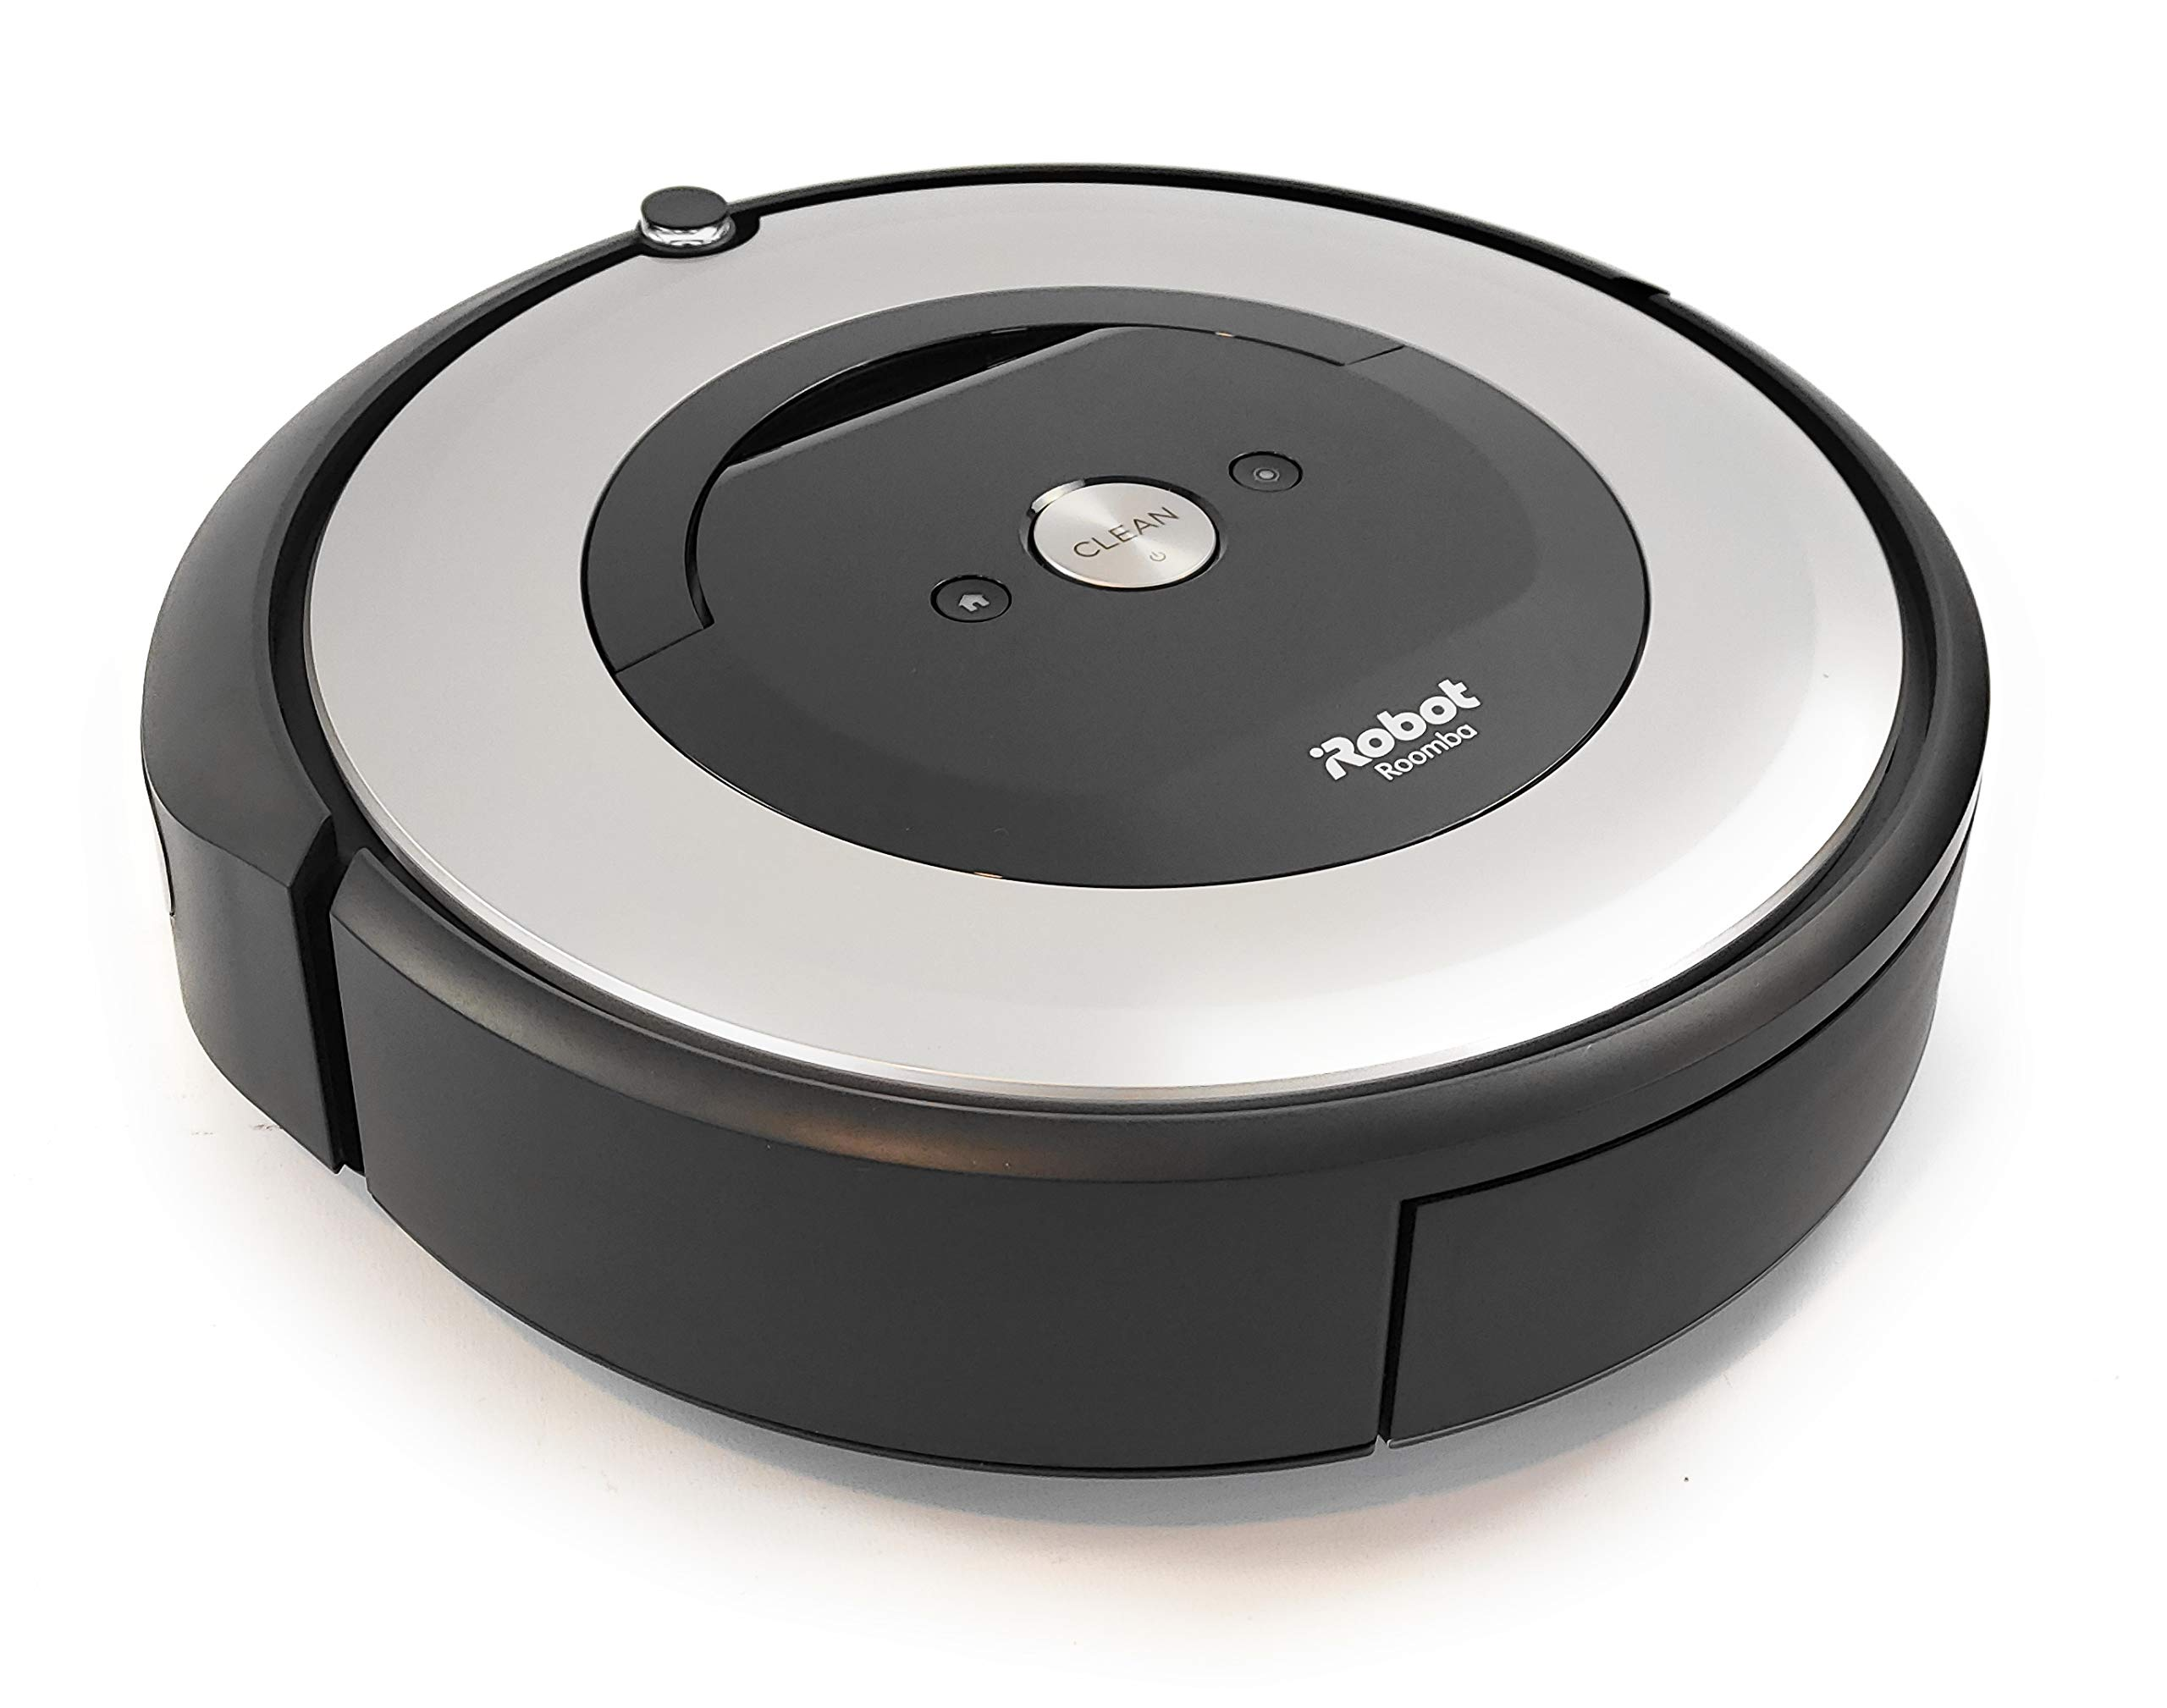
\includegraphics[width=0.5\textwidth]{figures/cap_1/roomba.jpg}
    \caption{Aspiradora autónoma}
    \label{fig:roomba}
\end{figure}

\begin{figure}[H]
    \centering
    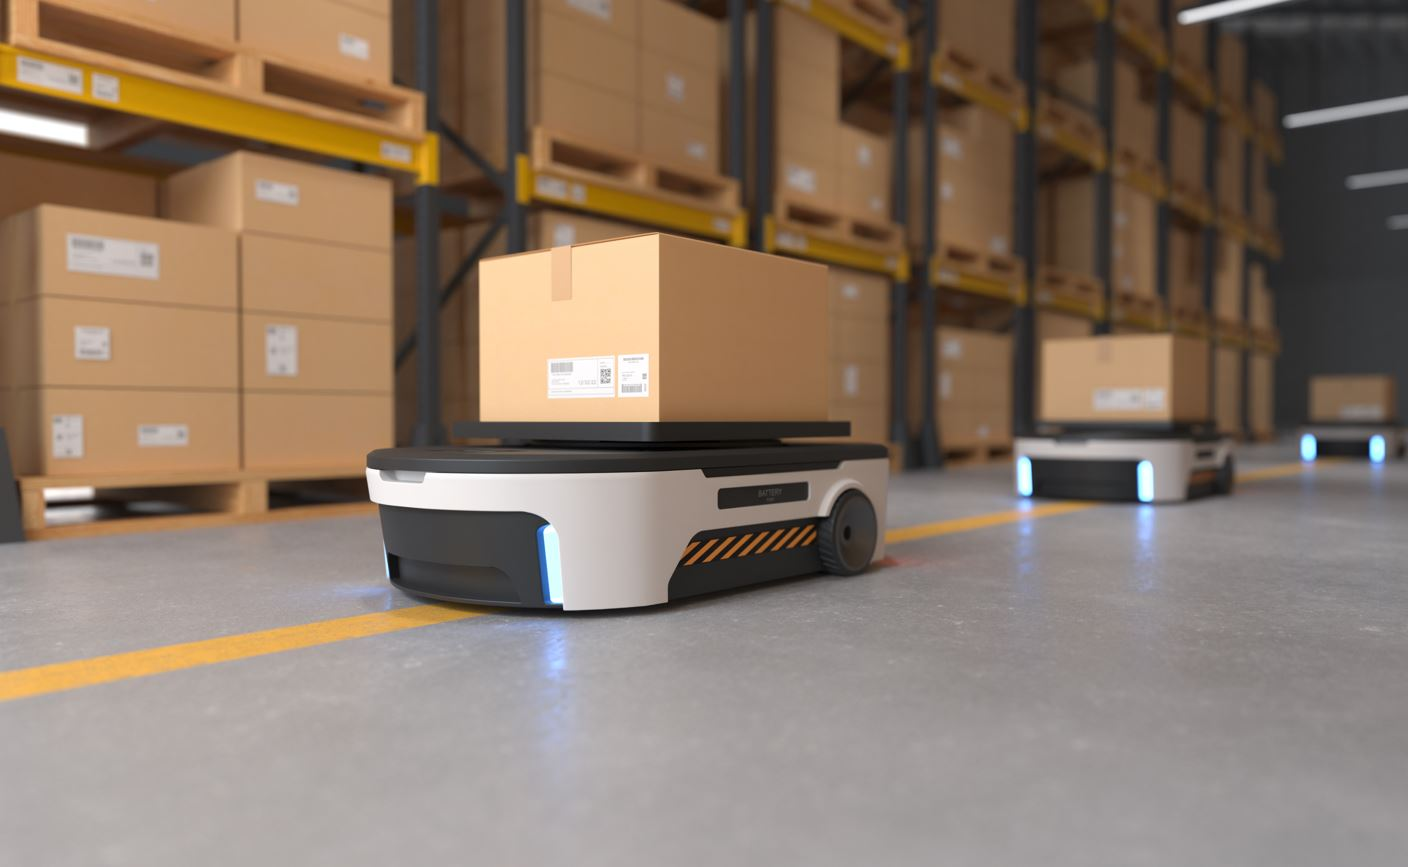
\includegraphics[width=0.7\textwidth]{figures/cap_1/agv.jpeg}
    \caption{Robot logístico AGV}
    \label{fig:agv}
\end{figure}

\begin{figure}[H]
    \centering
    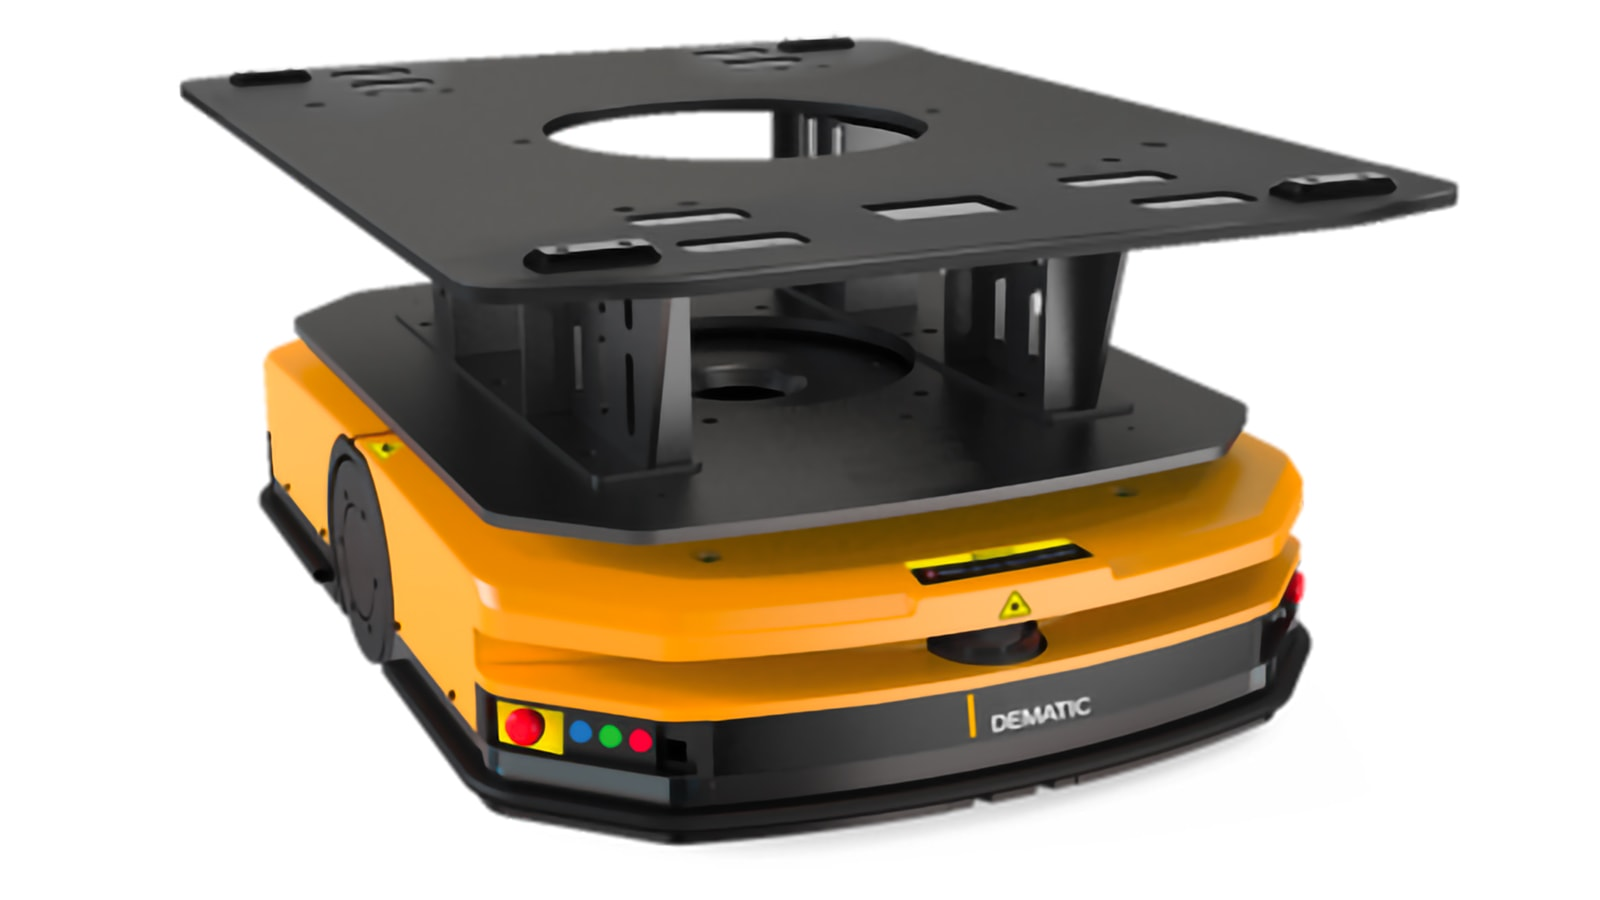
\includegraphics[width=0.7\textwidth]{figures/cap_1/amr.jpg}
    \caption{Robot logístico AMR}
    \label{fig:amr}
\end{figure}

\begin{figure}[H]
    \centering
    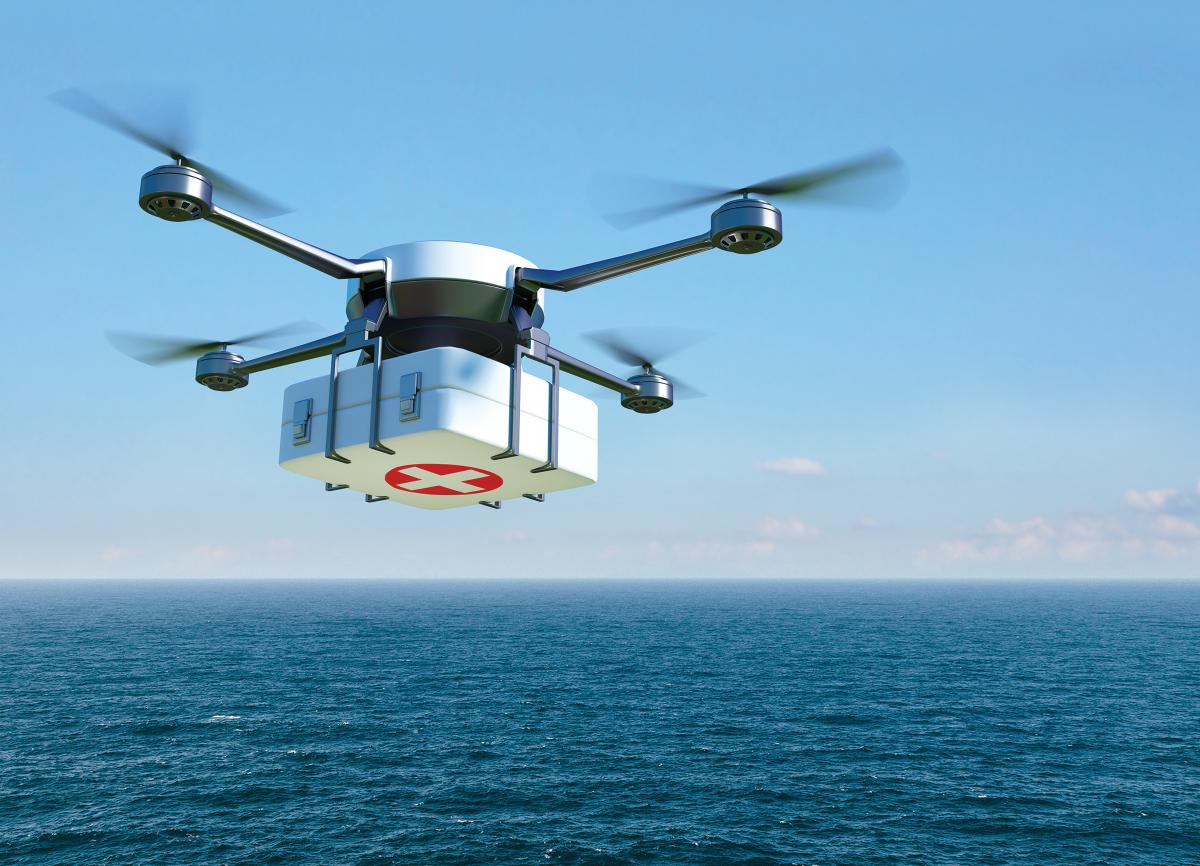
\includegraphics[width=0.7\textwidth]{figures/cap_1/dron.jpg}
    \caption{Dron de rescate}
    \label{fig:dron}
\end{figure}

\begin{figure}[H]
    \centering
    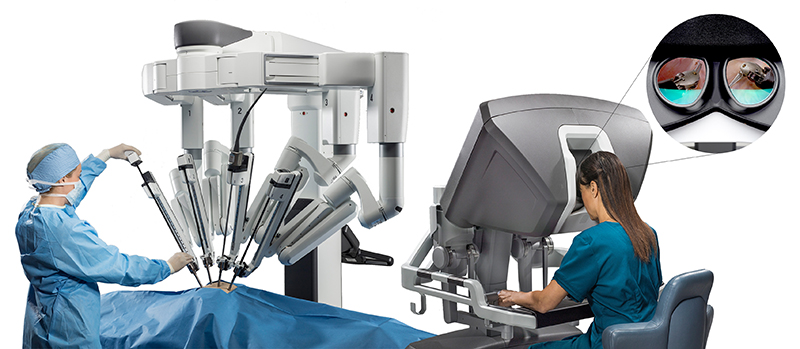
\includegraphics[width=0.9\textwidth]{figures/cap_1/davinci.jpg}
    \caption{Robot Da Vinci}
    \label{fig:davinci}
\end{figure}

Estos robots también se conocen como robots de consumo, y pueden clasificarse en dos categorías: personales y profesionales. Los primeros operan en el entorno doméstico, mientras que los segundos están diseñados para entornos empresariales, como fábricas, almacenes o zonas de construcción.

Es importante no confundirlos con los robots industriales, que suelen ser brazos robóticos fijos dedicados a realizar tareas repetitivas en un entorno controlado, como una línea de producción. Una excepción son los cobots (robots colaborativos), que están diseñados para interactuar directamente con personas en el ámbito industrial. Un ejemplo de estos robots son los de la empresa \textit{Universal Robots}\footnote{\url{https://www.universal-robots.com/es/}}, cuyos robots se muestran en la \autoref{fig:ur}.

\begin{figure}[H]
    \centering
    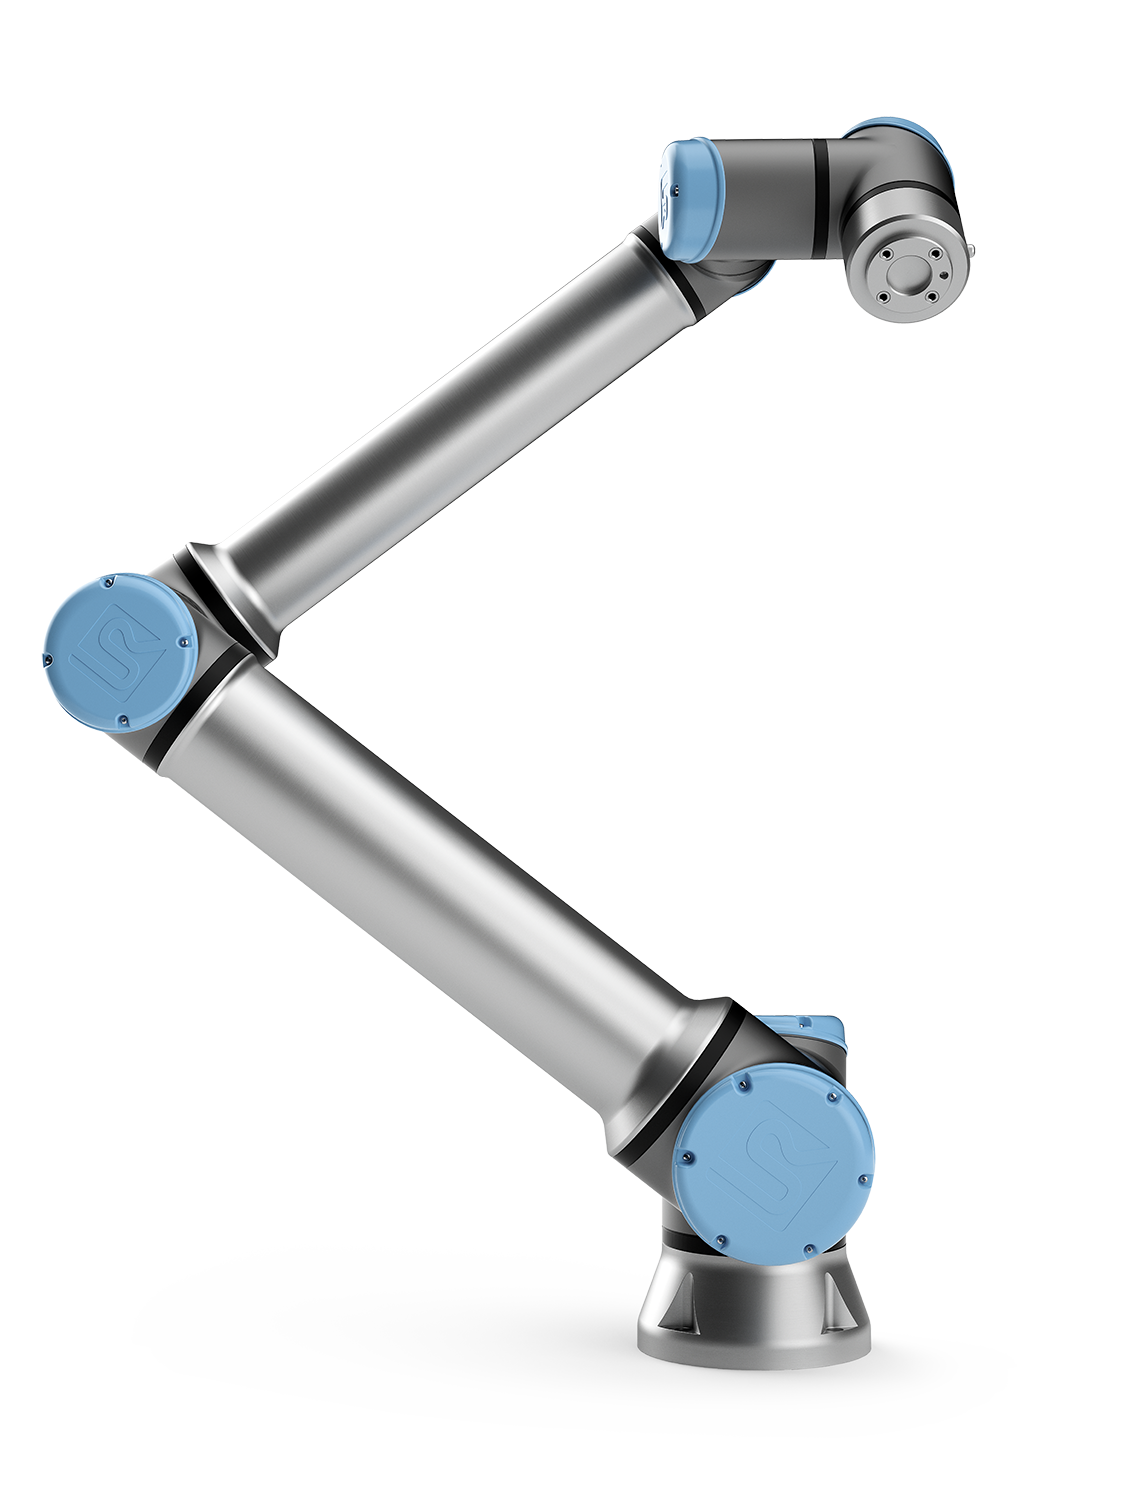
\includegraphics[height=0.7\textwidth]{figures/cap_1/ur10e.png}
    \caption{UR10e, Robot Colaborativo de Universal Robots}
    \label{fig:ur}
\end{figure}

A diferencia de los robots industriales, los robots de servicio o consumo deben desenvolverse en entornos no controlados, e incluso potencialmente hostiles. Además, no están necesariamente limitados a una sola tarea, ya que pueden adaptarse para realizar múltiples funciones y operar en distintos contextos.

\section{Robots Humanoides}

Dentro de los robots de servicio, destacan los robots humanoides, aquellos con la forma de su cuerpo construido para parecerse al cuerpo humano. Estos robots son especialmente interesantes a la hora de realizar tareas que ayuden a las personas. ESto es gracias a su diseño, que los hace lo suficientemente versátiles a la hora de realizar dichas tareas. Esto es porque pueden hacer las mismas tareas que las personas, al tener la misma complexión y anatomía.

Un ejemplo de este tipo de robots es el famoso Atlas\footnote{\url{https://bostondynamics.com/atlas/}}, de Boston Dynamics\footnote{\url{https://bostondynamics.com/}}. Este robot es completamente eléctrico y ha demostrado ser un robot extremadamente ágil, aunque no tanto como su predecesor, el robot Atlas hidráulico, capaz de moverse por entornos extremadamente complicados e incluso hacer acrobacias complejas. Ambos robots pueden verse en la \autoref{fig:atlas_electrico} y en la \autoref{fig:atlas_hidraulico}, respectivamente. También se adjuntan vídeos\footnote{\url{https://www.youtube.com/watch?v=I44_zbEwz_w}}\footnote{\url{https://www.youtube.com/watch?v=tF4DML7FIWk}} de lo que estos robots son capaces de hacer, también respectivamente.

\begin{figure}[H]
    \centering
    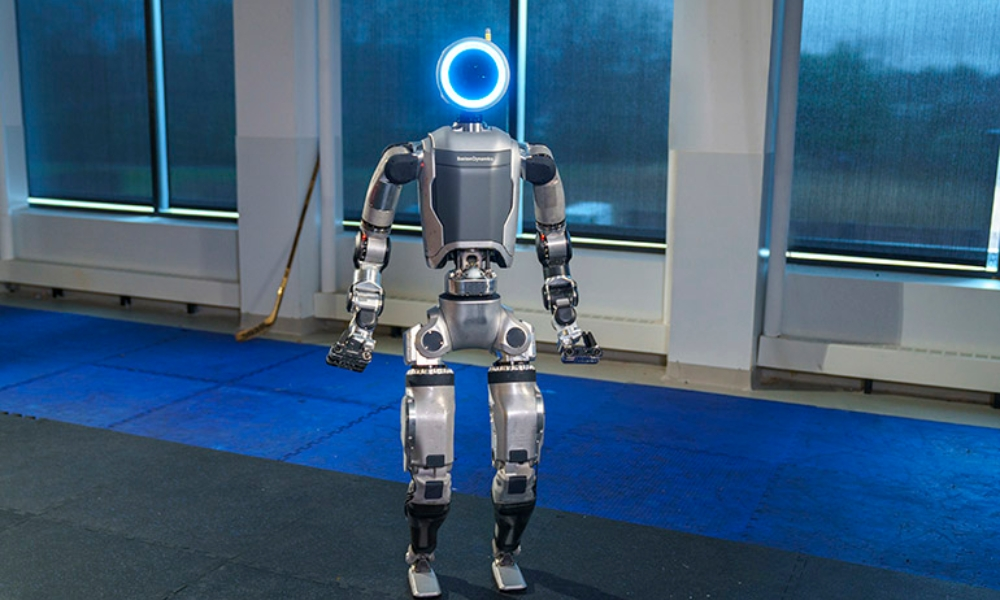
\includegraphics[width=0.8\textwidth]{figures/cap_1/atlas_electrico.jpg}
    \caption{Robot Atlas Eléctrico}
    \label{fig:atlas_electrico}
\end{figure}

\begin{figure}[H]
    \centering
    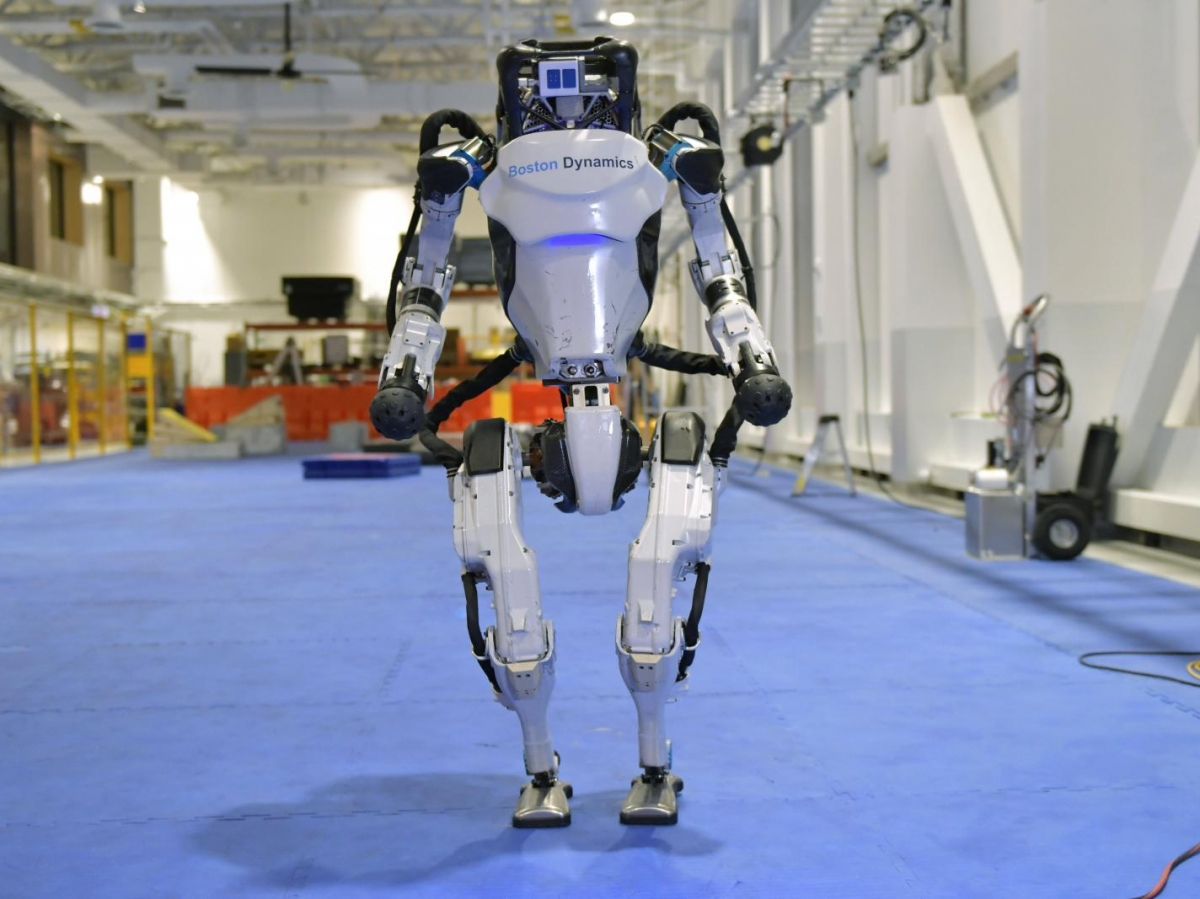
\includegraphics[width=0.8\textwidth]{figures/cap_1/atlas_hidraulico.jpg}
    \caption{Robot Atlas Hidráulico}
    \label{fig:atlas_hidraulico}
\end{figure}

Pero Atlas no es el único robot humanoide que existe, también tenemos al robot de Tesla\footnote{\url{https://www.tesla.com/es_es}}, Optimus\footnote{\url{https://www.tesla.com/es_es/we-robot}}, que también ha demostrado ser un robot bastante potente capaz de hacer varias tareas. Se muestra a continuación este robot en la \autoref{fig:optimus} y un vídeo\footnote{\url{https://www.youtube.com/watch?v=cpraXaw7dyc}} para conocer mejor a este robot.  

\begin{figure}[H]
    \centering
    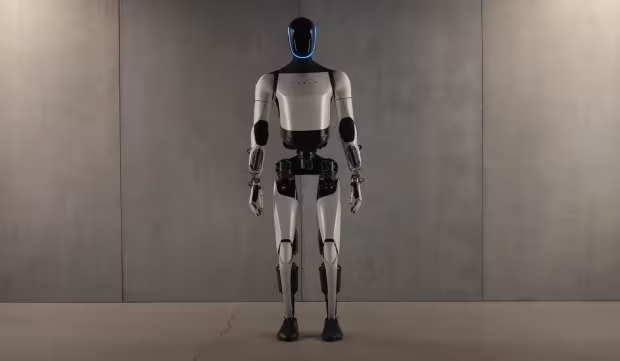
\includegraphics[width=0.8\textwidth]{figures/cap_1/optimus.jpg}
    \caption{Robot Optimus}
    \label{fig:optimus}
\end{figure}

Estos robots son demostradores, que sirven para enseñar hasta dónde somos capaces de llegar con la tecnología más puntera (pero no quiere decir que en el futuro se conviertan en robots de servicio masivos, cosa que aún nos queda un poco lejos).

Robots de servicio humanoides hay pocos, sin embargo, sí existen. Como ejemplo de este hecho tenemos a Digit\footnote{\url{https://www.agilityrobotics.com/solution}}, de Agility Robotics\footnote{\url{https://www.agilityrobotics.com/}}, un robot humanoide destinado a la logística que ha demostrado cumplir bastante bien con su tarea; para demostrarlo, se deja a continuación un vídeo\footnote{\url{https://www.youtube.com/watch?v=q8IdbodRG14}} donde lo vemos actuar. También se adjunta una fotografía de este robot en la \autoref{fig:digit}.

\begin{figure}[H]
    \centering
    \includegraphics[width=0.8\textwidth]{figures/cap_1/digit.jpg}
    \caption{Robot Digit}
    \label{fig:digit}
\end{figure}

Sin embargo, aunque estos robots son construibles en la vida real, suponen una dificultad muy alta, ya que hay que tener en cuenta muchos factores y desafíos.

Estos desafíos residen especialmente en la locomoción, ya que, al moverse mediante piernas, deben estables tanto estática cómo dinámicamente. También deben tener una anatomía adecuada y un aspecto amigable para los humanos, lo que conlleva esquivar \textit{el valle inquietante}, un punto en el que los robots son tan realistas que causan rechazo, e incluso miedo en algunos casos. Es por eso que los que hemos visto anteriormente no son tan antropomórficos ni realistas. 

También como desafío están el tamaño y el peso del robot, que, al ser de un tamaño grande, hay que compensar los pesos adecuadamente para conseguir esa estabilidad estática que se mencionaba anteriormente. En cuanto a la estabilidad dinámica, esto requiere mucho tiempo de entrenamiento del robot en cuanto a modos de caminar, cosa que se suele hacer mediante entrenamiento por refuerzo en simuladores.

Cómo último ejemplo de robot humanoide se hace referencia al robot NAO\cite{pagina_nao}, de Aldebaran, ahora Softbank Robotics\footnote{\url{https://us.softbankrobotics.com/}}. Protagonista de este TFG.

Este robot es el pequeño humanoide de 4,3 kg de peso y 58 cm de altura que se puede ver en la \autoref{fig:nao}.

\begin{figure}[H]
    \centering
    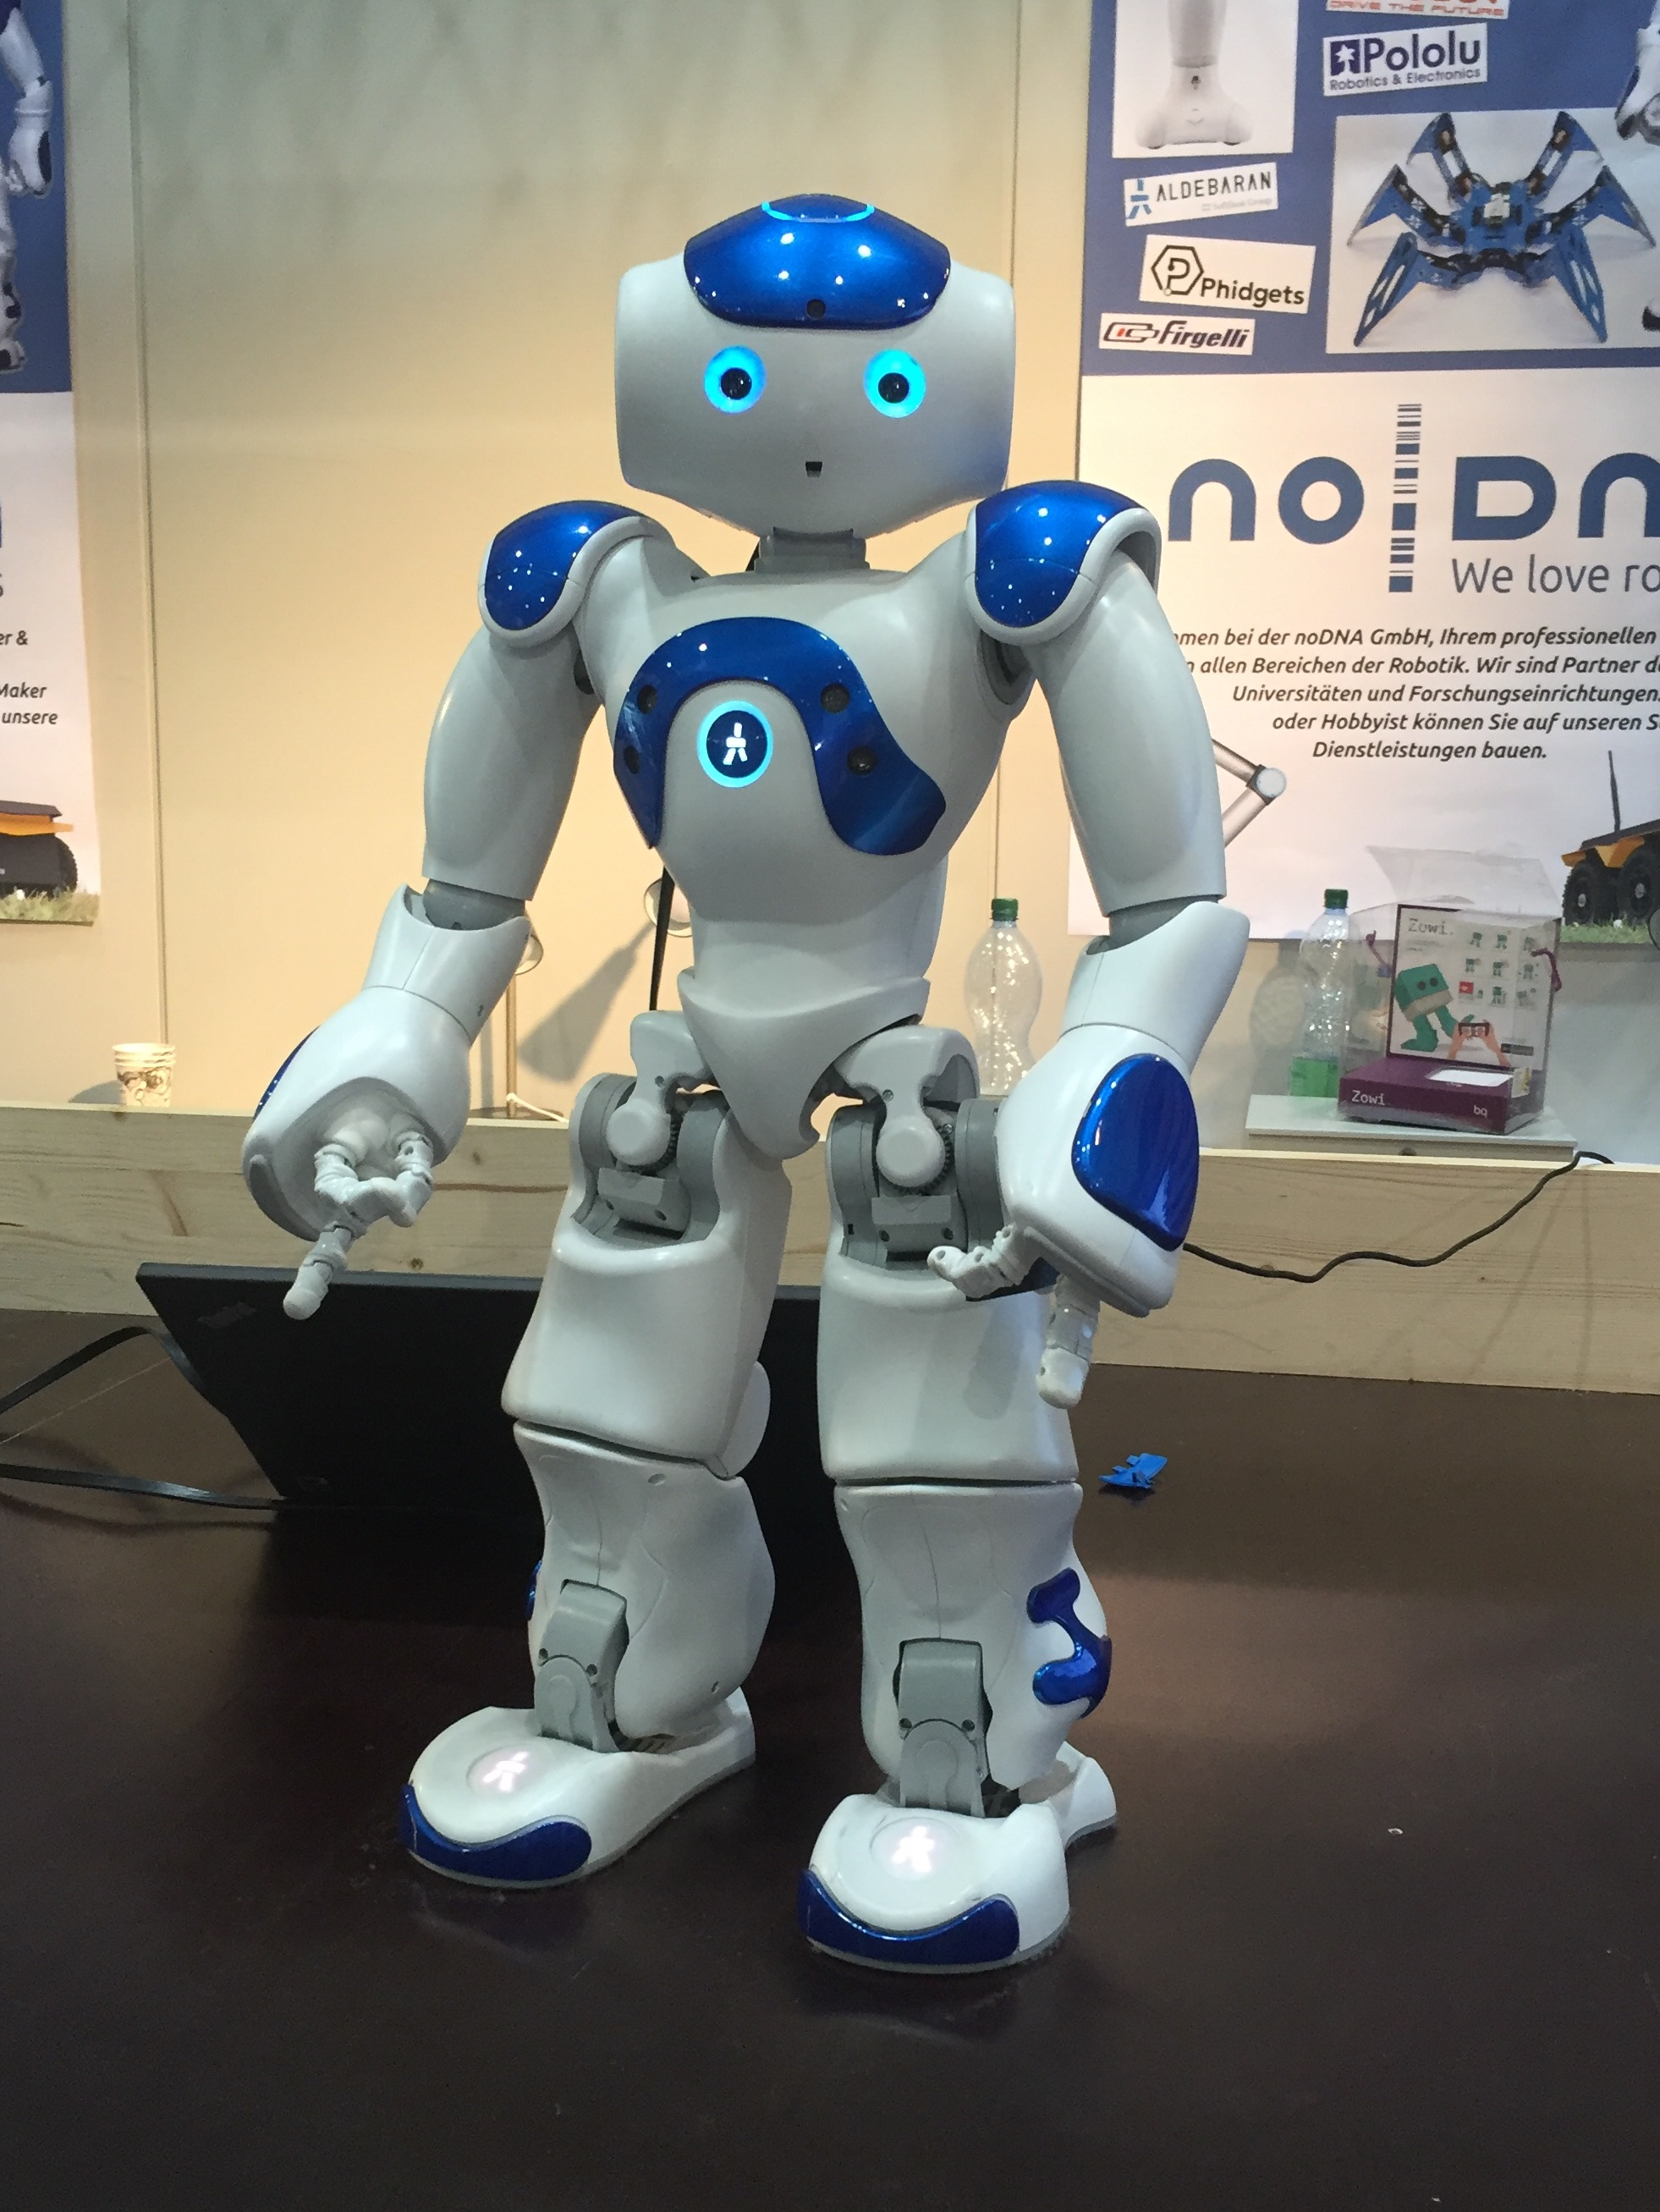
\includegraphics[width=0.5\textwidth]{figures/cap_1/nao.jpg}
    \caption{Robot NAO}
    \label{fig:nao}
\end{figure}

Sin embargo, este robot no es un robot de servicios. Es un robot principalmente educativo, destinado a que las personas aprendan las bases de la robótica y la programación mientras lo usan, además de ser divertido para los niños e interesante para la investigación. De hecho, este robot fue la liga de hardware estandard dentro de la RoboCup soccer\footnote{\url{https://www.robocup.org/leagues/5}} durante 17 años consecutivos, desde 2008 hasta 2024.

Este robot también ha protagonizado muchos trabajos de fin de grado anteriores, por ser el humanoide más accesible tanto por nuestra universidad (por tenerlo en el laboratorio), como por los estudiantes individualmente al poder acceder a su modelo simulado. Ejemplos de dichos trabajos pueden apreciarse en \cite{tfg_caminata_nao}, y  \cite{tfg_caminatas_ondas}, dónde se utiliza este robot para explorar  modos de caminar, un problema muy común en humanoides y muy interesante para investigar debido a su elevada complejidad.

Cabe destacar también que este robot es muy versátil a la hora de programarlo, ya que se puede optar por su forma predeterminada mediante Naoqui\footnote{\url{http://doc.aldebaran.com/1-14/dev/naoqi/index.html}}, un \textit{framework} específico para prgramar al robot mediante programación visual que puede verse en la \autoref{fig:naoqui}. Pero también ofrece la posibilidad de programarlo mediante el uso de ROS2, como se hará en este TFG o bien utilizando otros medios como por ejemplo el simulador Webots, al que haremos refrencia en el capítulo \ref{cap:herramientas}.

\begin{figure}[H]
    \centering
    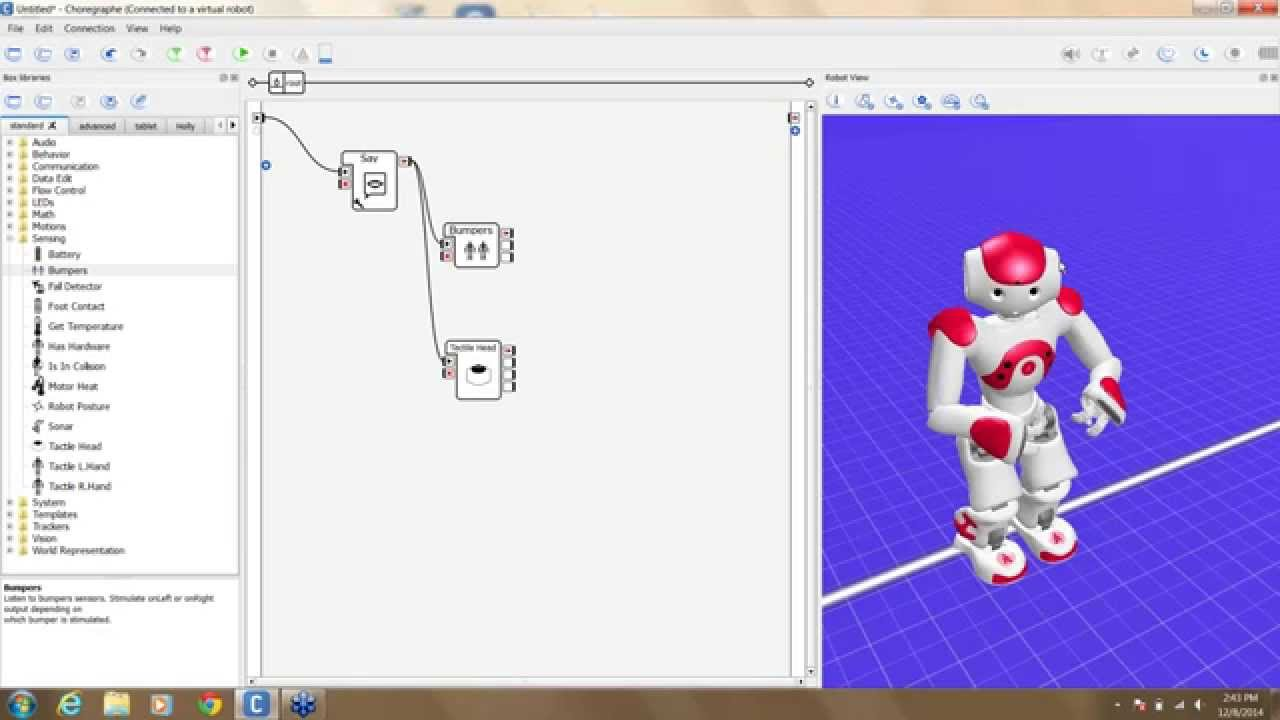
\includegraphics[width=1\textwidth]{figures/cap_1/naoqui.jpg}
    \caption{Lenguaje Naoqui}
    \label{fig:naoqui}
\end{figure}

\section{Simuladores Robóticos}

Los simuladores son aplicaciones software que permiten emular \textit{via software} de manera realista al robot y su entorno, lo que los convierte en una herramienta extremadamente útil a la hora de construir todo tipo de robots, ya que evitan posibles catástrofes en la realidad a la hora de usarlos, por ejemplo, si un robot cae en el entorno simulado, sus componentes reales quedarán a salvo. Es por eso por lo que tienen mucha importancia a la hora del desarrollo de robots humanoides, debido a su elevado coste y complicación a la hora de construirlos. Los simuladores también son útiles para entrenar dichos robots en diferentes ámbitos y escenarios, para así brindarles la máxima versatilidad posible y que puedan realizar casi cualquier tarea que podría hacer un humano.

Existen muchos simuladores robóticos, entre los que destacan el simulador de NVIDIA\footnote{\url{https://www.nvidia.com/es-es/}}, Isaac Sim\footnote{\url{https://developer.nvidia.com/isaac/sim}}, capaz de entrenar un robot para que aprenda a caminar en sólamente 2 horas, según lo indicado por CyberRobo en la plataforma X\footnote{\url{https://x.com/CyberRobooo/status/1921252216330912032}}. 

Otro simulador muy presente en la actualidad es Coppelia Sim\footnote{\url{https://www.coppeliarobotics.com/}}, un simulador utilizado en la industria, la educación y la investigación. Originalmente fue desarrollado dentro del departamento de I+D de Toshiba\footnote{\url{https://www.toshiba.es/}} y actualmente está siendo desarrollado y mantenido activamente por Coppelia Robotics AG\footnote{\url{https://github.com/CoppeliaRobotics}}, una pequeña empresa ubicada en Zúrich, Suiza. Este simulador ha resultado muy útil para simulación de robots móviles con navegación autónoma, Robots que usan SLAM para mapear un entorno, brazos robóticos con \textit{pick and place}, e incluso simulación de robots humanoides caminantes.

También existe el simulador Webots, un simulador \textit{opensource} educativo en el que se hará más incapié en el capítulo \ref{cap:herramientas}.

Por último, destaca también Gazebo, simulador específico para ROS2, muy potente y además \textit{opensource}. Éste es el simulador que se utilizará para el desarrollo de este TFG. Se hablará más en profundidad sobre él en el Capítulo \ref{cap:herramientas}.

Todo lo expuesto en este capítulo ha sido clave para decidir como objetivo dotar al robot NAO simulado en Gazebo de una librería de coordinación de actuadores que le permita caminar (especialmente por el desafío técnico que supone) y, además, programar una aplicación en el contexto de un invernadero como validación experimental de la biblioteca de movimientos y de su potencial uso como robot de servicio.